% Nerdfit dynamics — color-coded equation figures (see MODEL.md)
% Compile: pdflatex model-equations.tex  (needs amsmath, xcolor, tikz, standalone)
% Docker:  docker run --rm -v "$PWD":/work -w /work texlive/texlive:latest pdflatex model-equations.tex

% Multiple pages: one PDF with one figure per page (for PNG export per page)
\documentclass[border=10pt,multi=tikzpicture]{standalone}
\standaloneenv{tikzpicture}

\usepackage{lmodern}
\usepackage{amsmath,amssymb}
\usepackage{xcolor}
\usepackage{tikz}
\usetikzlibrary{arrows.meta,positioning,calc}

\newcommand{\ind}{\mathbf{1}}

% --- Phenomenon palette (aligned with MODEL.md / PHENOMENA.md) ---
\definecolor{st}{HTML}{1B2631}      % state variables
\definecolor{hb}{HTML}{1B7F6A}      % habit & automaticity
\definecolor{mv}{HTML}{C45C26}      % motivation & reward
\definecolor{ef}{HTML}{5C4D8A}      % effort / opportunity cost
\definecolor{ex}{HTML}{6B4C9A}      % expectation excess & calibration
\definecolor{id}{HTML}{2874A6}      % identity & self-concept
\definecolor{cx}{HTML}{7D6608}      % behavioral complexity
\definecolor{fn}{HTML}{AF601A}      % fantasy / indulgence (Oettingen)
\definecolor{cl}{HTML}{B03A2E}      % collapse & disinhibition (false hope, WTH)
\definecolor{ct}{HTML}{1F618D}      % context: stress, social, implementation intentions
\definecolor{mt}{HTML}{566573}      % meta-control (Carver–Scheier velocity, gates)

\newcommand{\St}[1]{\ensuremath{\textcolor{st}{\mathbf{#1}}}}
\newcommand{\Hb}[1]{\ensuremath{\textcolor{hb}{#1}}}
\newcommand{\Mv}[1]{\ensuremath{\textcolor{mv}{#1}}}
\newcommand{\Ef}[1]{\ensuremath{\textcolor{ef}{#1}}}
\newcommand{\Ex}[1]{\ensuremath{\textcolor{ex}{#1}}}
\newcommand{\Id}[1]{\ensuremath{\textcolor{id}{#1}}}
\newcommand{\Cx}[1]{\ensuremath{\textcolor{cx}{#1}}}
\newcommand{\Fn}[1]{\ensuremath{\textcolor{fn}{#1}}}
\newcommand{\Cl}[1]{\ensuremath{\textcolor{cl}{#1}}}
\newcommand{\Mt}[1]{\ensuremath{\textcolor{mt}{#1}}}
\newcommand{\Ct}[1]{\ensuremath{\textcolor{ct}{\text{#1}}}}
\newcommand{\Ctii}{\ensuremath{\textcolor{ct}{\mathit{ii}}}}
\newcommand{\Ctx}[1]{\textcolor{ct}{\textsf{#1}}}

\newcommand{\legendsquare}[2]{\textcolor{#1}{\rule{10pt}{10pt}}~#2}

\begin{document}

% ==================== 0. Color key ====================
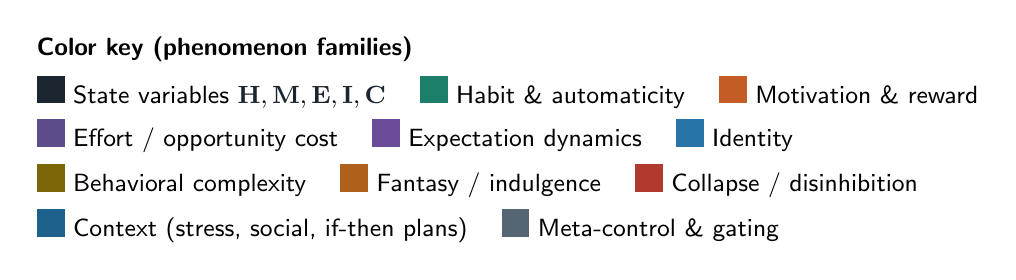
\begin{tikzpicture}
  \node[anchor=west, align=left, font=\small\sf] (L) at (0,0) {%
    \textbf{Color key (phenomenon families)}\\[4pt]
    \legendsquare{st}{State variables $\St{H},\St{M},\St{E},\St{I},\St{C}$}
    \quad \legendsquare{hb}{Habit \& automaticity}
    \quad \legendsquare{mv}{Motivation \& reward}\\[3pt]
    \legendsquare{ef}{Effort / opportunity cost}
    \quad \legendsquare{ex}{Expectation dynamics}
    \quad \legendsquare{id}{Identity}\\[3pt]
    \legendsquare{cx}{Behavioral complexity}
    \quad \legendsquare{fn}{Fantasy / indulgence}
    \quad \legendsquare{cl}{Collapse / disinhibition}\\[3pt]
    \legendsquare{ct}{Context (stress, social, if-then plans)}
    \quad \legendsquare{mt}{Meta-control \& gating}
  };
\end{tikzpicture}

% ==================== 1. Behavioral trigger ====================
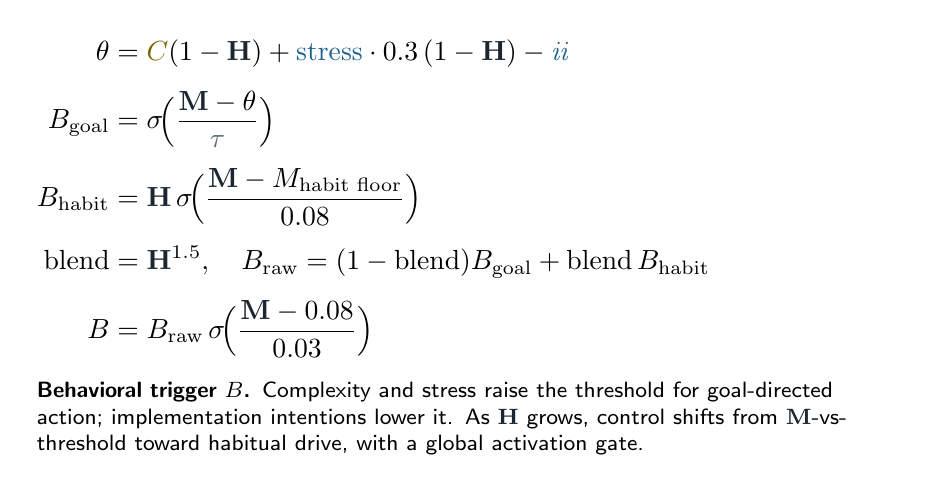
\begin{tikzpicture}
  \node[anchor=west] (eq) at (0,0) {$
    \begin{aligned}
      \theta &= \Cx{C}(1-\St{H}) + \Ct{stress}\cdot 0.3\,(1-\St{H}) - \Ctii \\[0.35em]
      B_{\text{goal}} &= \sigma\!\Bigl(\dfrac{\St{M}-\theta}{\Mt{\tau}}\Bigr) \\[0.35em]
      B_{\text{habit}} &= \St{H}\,\sigma\!\Bigl(\dfrac{\St{M}-M_{\text{habit floor}}}{0.08}\Bigr) \\[0.35em]
      \text{blend} &= \St{H}^{1.5},\quad
      B_{\text{raw}} = (1-\text{blend})B_{\text{goal}} + \text{blend}\,B_{\text{habit}} \\[0.35em]
      B &= B_{\text{raw}}\,\sigma\!\Bigl(\dfrac{\St{M}-0.08}{0.03}\Bigr)
    \end{aligned}
  $};
  \node[anchor=north west, font=\footnotesize\sf, text width=11cm, align=left, yshift=-2pt]
    at (eq.south west) {%
    \textbf{Behavioral trigger $B$.}
    Complexity and stress raise the threshold for goal-directed action; implementation intentions lower it.
    As \St{H} grows, control shifts from \St{M}-vs-threshold toward habitual drive, with a global activation gate.};
\end{tikzpicture}

% ==================== 2. Fantasy ====================
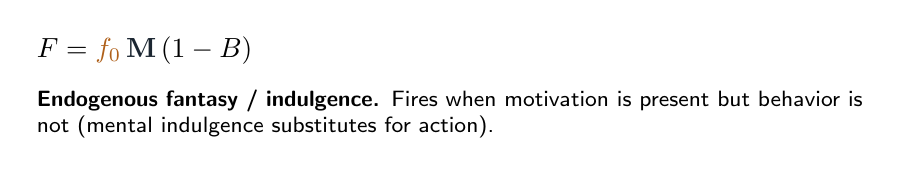
\begin{tikzpicture}
  \node[anchor=west] (eq) at (0,0) {$
    F = \Fn{f_0}\,\St{M}\,(1-B)
  $};
  \node[anchor=north west, font=\footnotesize\sf, text width=10.5cm, align=left, yshift=-2pt]
    at (eq.south west) {%
    \textbf{Endogenous fantasy / indulgence.}
    Fires when motivation is present but behavior is not (mental indulgence substitutes for action).};
\end{tikzpicture}

% ==================== 3. dH/dt ====================
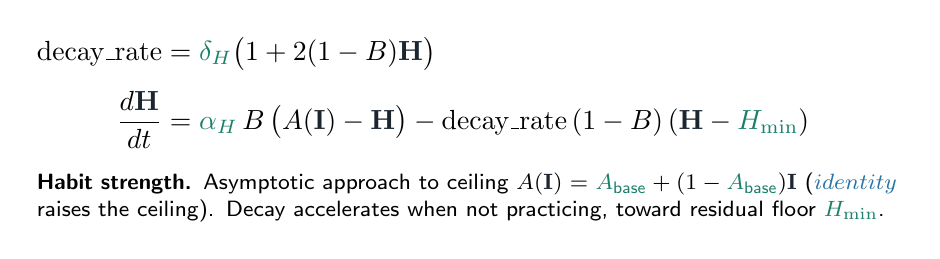
\begin{tikzpicture}
  \node[anchor=west] (eq) at (0,0) {$
    \begin{aligned}
      \text{decay\_rate} &= \Hb{\delta_H}\bigl(1 + 2(1-B)\St{H}\bigr) \\[0.35em]
      \dfrac{d\St{H}}{dt} &= \Hb{\alpha_H}\,B\,\bigl(A(\St{I})-\St{H}\bigr)
        - \text{decay\_rate}\,(1-B)\,(\St{H}-\Hb{H_{\min}})
    \end{aligned}
  $};
  \node[anchor=north west, font=\footnotesize\sf, text width=11cm, align=left, yshift=-2pt]
    at (eq.south west) {%
    \textbf{Habit strength.}
    Asymptotic approach to ceiling $A(\St{I})=\Hb{A_{\text{base}}}+(1-\Hb{A_{\text{base}}})\St{I}$ (\Id{identity} raises the ceiling).
    Decay accelerates when not practicing, toward residual floor \Hb{H_{\min}}.};
\end{tikzpicture}

% ==================== 4. dM/dt ====================
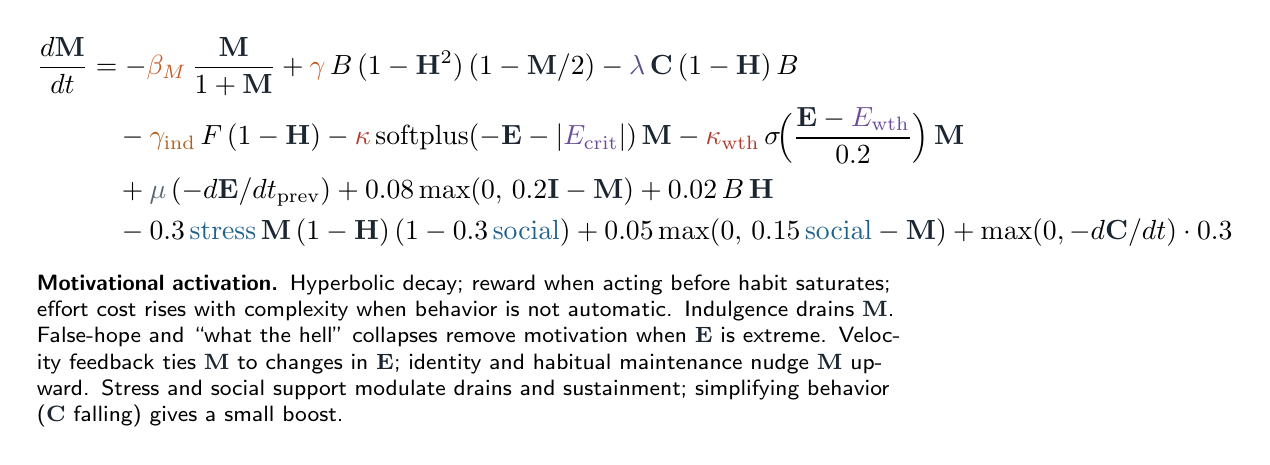
\begin{tikzpicture}
  \node[anchor=west] (eq) at (0,0) {$
    \begin{aligned}
      \dfrac{d\St{M}}{dt} &=
        -\Mv{\beta_M}\,\dfrac{\St{M}}{1+\St{M}}
        + \Mv{\gamma}\,B\,(1-\St{H}^2)\,(1-\St{M}/2)
        - \Ef{\lambda}\,\St{C}\,(1-\St{H})\,B \\
        &\quad - \Fn{\gamma_{\text{ind}}}\,F\,(1-\St{H})
        - \Cl{\kappa}\,\mathrm{softplus}(-\St{E}-|\Ex{E_{\text{crit}}}|)\,\St{M}
        - \Cl{\kappa_{\text{wth}}}\,\sigma\!\Bigl(\dfrac{\St{E}-\Ex{E_{\text{wth}}}}{0.2}\Bigr)\,\St{M} \\
        &\quad + \Mt{\mu}\,(-d\St{E}/dt_{\text{prev}})
        + 0.08\max(0,\,0.2\St{I}-\St{M})
        + 0.02\,B\,\St{H} \\
        &\quad - 0.3\,\Ct{stress}\,\St{M}\,(1-\St{H})\,(1-0.3\,\Ct{social})
        + 0.05\max(0,\,0.15\,\Ct{social}-\St{M})
        + \max(0,-d\St{C}/dt)\cdot 0.3
    \end{aligned}
  $};
  \node[anchor=north west, font=\footnotesize\sf, text width=11.2cm, align=left, yshift=-2pt]
    at (eq.south west) {%
    \textbf{Motivational activation.}
    Hyperbolic decay; reward when acting before habit saturates; effort cost rises with complexity when behavior is not automatic.
    Indulgence drains \St{M}. False-hope and ``what the hell'' collapses remove motivation when \St{E} is extreme.
    Velocity feedback ties \St{M} to changes in \St{E}; identity and habitual maintenance nudge \St{M} upward.
    Stress and social support modulate drains and sustainment; simplifying behavior (\St{C} falling) gives a small boost.};
\end{tikzpicture}

% ==================== 5. dE/dt ====================
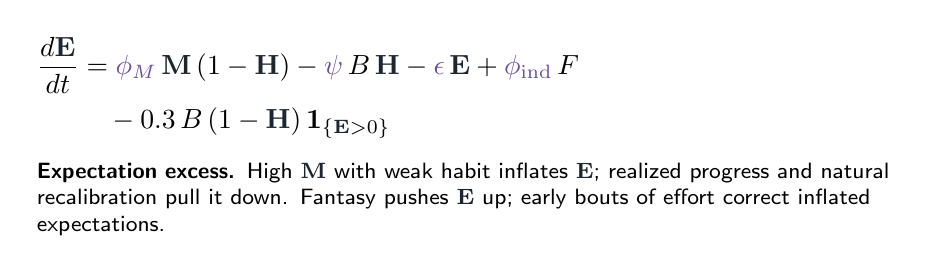
\begin{tikzpicture}
  \node[anchor=west] (eq) at (0,0) {$
    \begin{aligned}
      \dfrac{d\St{E}}{dt} &=
        \Ex{\phi_M}\,\St{M}\,(1-\St{H})
        - \Ex{\psi}\,B\,\St{H}
        - \Ex{\epsilon}\,\St{E}
        + \Ex{\phi_{\text{ind}}}\,F \\
        &\quad - 0.3\,B\,(1-\St{H})\,\ind_{\{\St{E}>0\}}
    \end{aligned}
  $};
  \node[anchor=north west, font=\footnotesize\sf, text width=11cm, align=left, yshift=-2pt]
    at (eq.south west) {%
    \textbf{Expectation excess.}
    High \St{M} with weak habit inflates \St{E}; realized progress and natural recalibration pull it down.
    Fantasy pushes \St{E} up; early bouts of effort correct inflated expectations.};
\end{tikzpicture}

% ==================== 6. dI/dt ====================
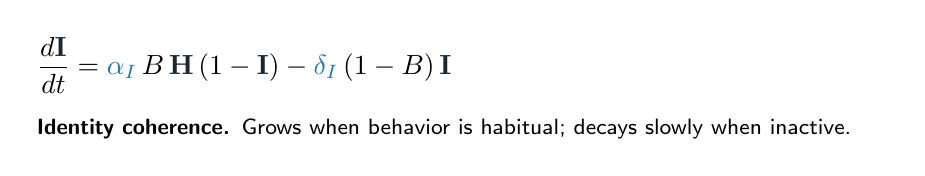
\begin{tikzpicture}
  \node[anchor=west] (eq) at (0,0) {$
    \dfrac{d\St{I}}{dt} =
      \Id{\alpha_I}\,B\,\St{H}\,(1-\St{I})
      - \Id{\delta_I}\,(1-B)\,\St{I}
  $};
  \node[anchor=north west, font=\footnotesize\sf, text width=10.8cm, align=left, yshift=-2pt]
    at (eq.south west) {%
    \textbf{Identity coherence.}
    Grows when behavior is habitual; decays slowly when inactive.};
\end{tikzpicture}

% ==================== 7. C_equil and dC/dt ====================
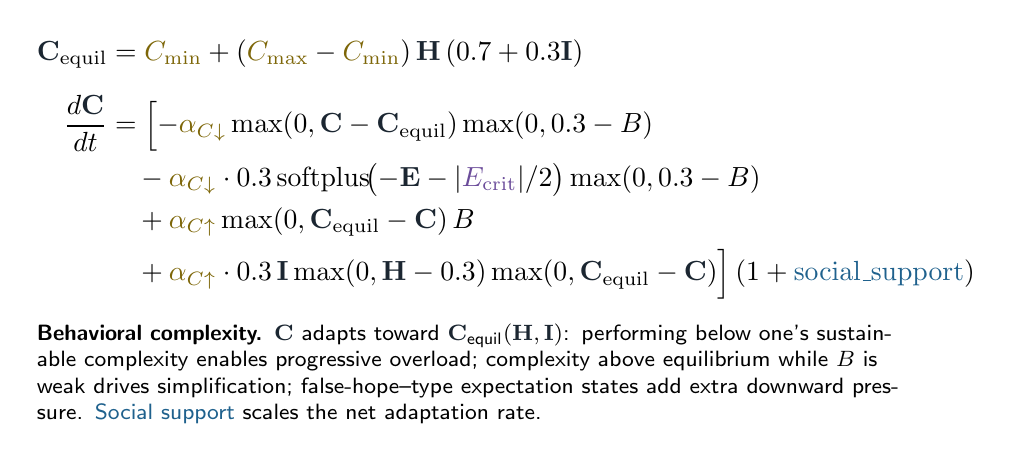
\begin{tikzpicture}
  \node[anchor=west] (eq) at (0,0) {$
    \begin{aligned}
      \St{C}_{\text{equil}} &= \Cx{C_{\min}} + (\Cx{C_{\max}}-\Cx{C_{\min}})\,\St{H}\,(0.7+0.3\St{I}) \\[0.5em]
      \dfrac{d\St{C}}{dt} &= \Bigl[
        -\Cx{\alpha_{C\downarrow}}\max(0,\St{C}-\St{C}_{\text{equil}})\max(0,0.3-B) \\
        &\quad -\Cx{\alpha_{C\downarrow}}\cdot 0.3\,\mathrm{softplus}\!\bigl(-\St{E}-|\Ex{E_{\text{crit}}}|/2\bigr)\max(0,0.3-B) \\
        &\quad +\Cx{\alpha_{C\uparrow}}\max(0,\St{C}_{\text{equil}}-\St{C})\,B \\
        &\quad +\Cx{\alpha_{C\uparrow}}\cdot 0.3\,\St{I}\max(0,\St{H}-0.3)\max(0,\St{C}_{\text{equil}}-\St{C})
      \Bigr]\,(1+\Ct{social\_support})
    \end{aligned}
  $};
  \node[anchor=north west, font=\footnotesize\sf, text width=11.2cm, align=left, yshift=-2pt]
    at (eq.south west) {%
    \textbf{Behavioral complexity.}
    \St{C} adapts toward $\St{C}_{\text{equil}}(\St{H},\St{I})$: performing below one's sustainable complexity enables progressive overload;
    complexity above equilibrium while $B$ is weak drives simplification; false-hope--type expectation states add extra downward pressure.
    \Ctx{Social support} scales the net adaptation rate.};
\end{tikzpicture}

% ==================== 8. Transient decay ====================
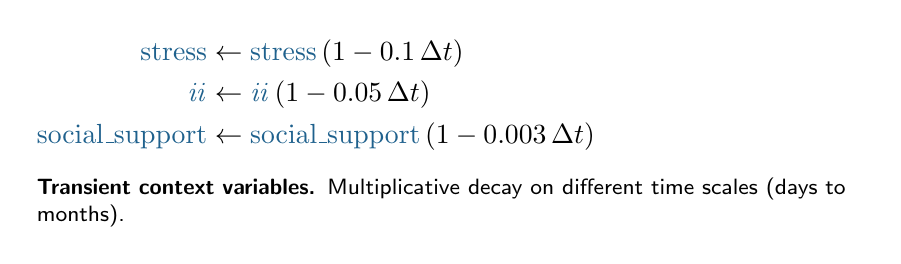
\begin{tikzpicture}
  \node[anchor=west] (eq) at (0,0) {$
    \begin{aligned}
      \Ct{stress} &\gets \Ct{stress}\,(1-0.1\,\Delta t) \\
      \Ctii &\gets \Ctii\,(1-0.05\,\Delta t) \\
      \Ct{social\_support} &\gets \Ct{social\_support}\,(1-0.003\,\Delta t)
    \end{aligned}
  $};
  \node[anchor=north west, font=\footnotesize\sf, text width=10.5cm, align=left, yshift=-2pt]
    at (eq.south west) {%
    \textbf{Transient context variables.}
    Multiplicative decay on different time scales (days to months).};
\end{tikzpicture}

\end{document}
